\documentclass[a4paper]{article}
\usepackage{svn-multi}
% Version control information:
\svnidlong
{$HeadURL: https://practicas-derive.googlecode.com/svn/trunk/concepto_derivada.tex $}
{$LastChangedDate: 2008-11-13 12:37:02 +0100 (jue, 13 nov 2008) $}
{$LastChangedRevision: 3 $}
{$LastChangedBy: asalber $}
\svnid{$Id: concepto_derivada.tex 3 2008-11-13 11:37:02Z asalber $}
\pdfinfo{/CreationDate (D:\svnpdfdate)}
\svnRegisterAuthor{alf}{Alfredo Sánchez Alberca}

\usepackage[spanish]{babel}
\usepackage[utf8x]{inputenc}
\usepackage{amsmath}
\usepackage{macros}
\usepackage[dvips]{graphicx}
\usepackage{enumitem}
\usepackage{subfigure}
\usepackage[small,bf]{caption2}
\usepackage[top=3cm, bottom=3cm, left=2.54cm, right=2.54cm]{geometry}
\usepackage{fancyhdr}
\pagestyle{fancy}

\lhead{\textsc{Universidad San Pablo CEU}} \rhead{\textsl{\textsf{Departamento de Métodos Cuantitativos}}}
\renewcommand{\headrulewidth}{0pt}
\renewcommand{\floatpagefraction}{.8}
\renewcommand{\textfraction}{.1}
\setcaptionwidth{\textwidth} \addtolength{\captionwidth}{-40pt}
\captionstyle{indent} \setlength\captionindent{\parindent}

\makeatletter
\let\savees@listquot\es@listquot
\def\es@listquot{\protect\savees@listquot}
\makeatletter

\begin{document}
\sloppy
\practica{Práctica de Cálculo con Derive}{Derivadas}

\bigskip
\section*{Fundamentos Teóricos}
El concepto de derivada es uno de los más importantes del Cálculo pues resulta
de gran utilidad en el estudio de funciones y tiene multitud de aplicaciones.
En esta práctica se introduce este concepto y se muestra cómo calcular derivadas con Derive.

\subsection*{Tasa de variación media}
Cuando queremos conocer la variación que experimenta una función real $y=f(x)$ en un intervalo $[a,b]$, se calcula la diferencia $f(b)-f(a)$ que se conoce como \emph{incremento} de $y$, y se nota $\Delta y[a,b]$, aunque a veces, simplemente se escribe $\Delta y$. Por ejemplo, si tenemos un móvil cuya posición en cada instante $t$ viene dada por la función $y=f(t)=t^2$, donde $y$ se mide en metros y $t$ se mide en segundos, entonces el camino recorrido durante el intervalo de tiempo que transcurre desde el segundo 2 hasta el segundo 5, será 
\[\Delta y[2,5]=f(5)-f(2)=5^2-2^2=25-4=21 \textrm{ m}.\].

Muchas veces resulta interesante comparar la variación que experimenta la función $y$ con relación a la variación que experimenta su argumento $x$ en un intervalo $[a,a+\Delta x]$. Esto viene dado por la \emph{tasa de variación media}, que define como
\[
\textrm{TVM} f[a,a+\Delta x]=\frac{\Delta y}{\Delta x}=\frac{f(a+\Delta x)-f(a)}{\Delta x}.
\]

Así, en el ejemplo anterior, la tasa de variación media de la función que determina la posición del móvil en el intervalo $[2,5]$ es
\[\textrm{TVM} f[2,5]=\frac{\Delta y}{\Delta x}=\frac{f(5)-f(2)}{5-2}=\frac{21}{3}=7\textrm{ m/s},\]
que en realidad es la velocidad media del móvil durante ese intervalo de tiempo.

Desde el punto de vista geométrico, la tasa de variación media de $f$ en el intervalo $[a , a+\Delta x]$ es la pendiente de la recta secante a $f$ en los puntos $(a , f(a))$ y $(a+\Delta x, f(a+\Delta x))$, tal y como se muestra en la figura~\ref{g:secante}.

\begin{figure}[h!]
\begin{center}
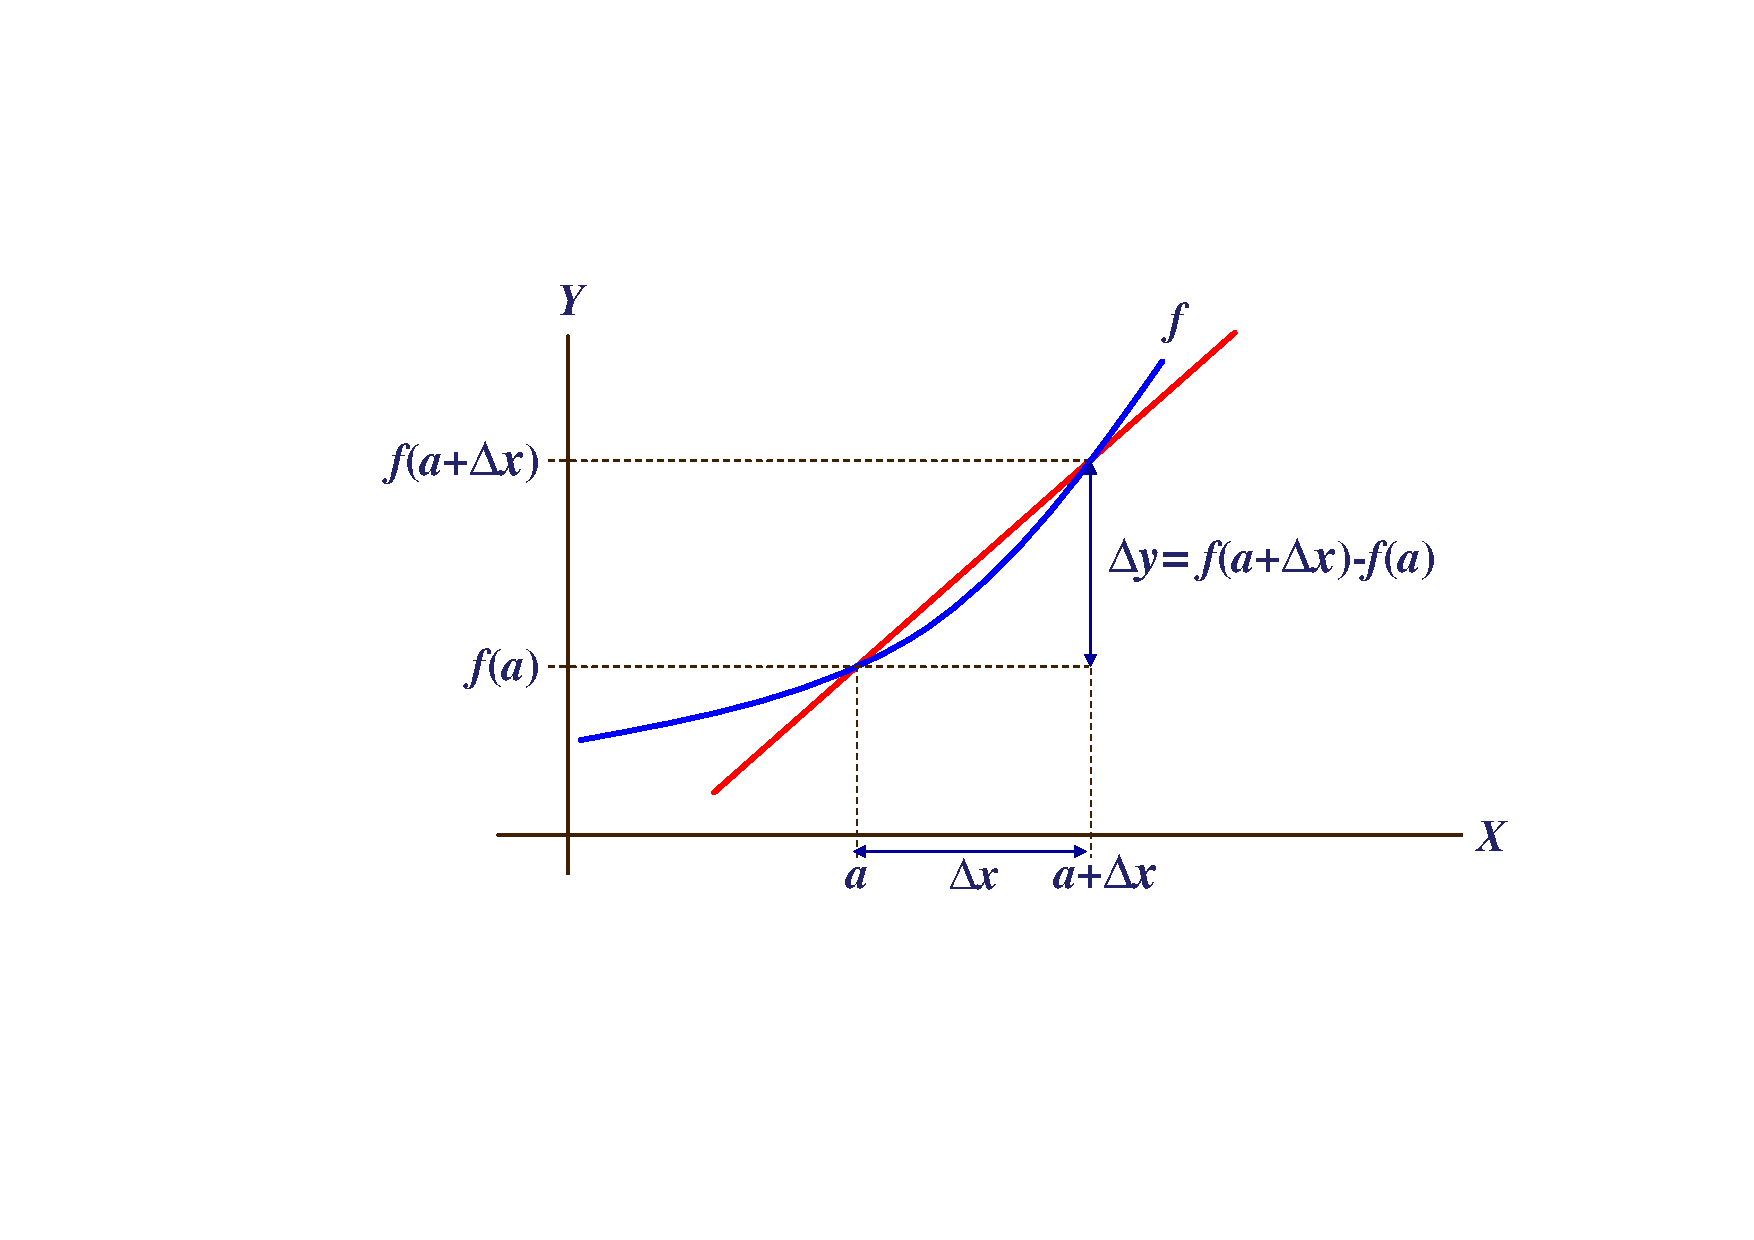
\includegraphics[scale=0.5]{secante}
\caption{La tasa de variación media como la pendiente de la 
recta secante a una función en dos puntos.}
\label{g:secante}
\end{center}
\end{figure}


\subsection*{Tasa de variación instantánea y derivada}
En muchas ocasiones, es interesante estudiar la tasa de variación que experimenta una función, no en un intervalo, sino en un punto. Por ejemplo, si tenemos una función que depende del tiempo, conocer la tasa de variación de la función en un determinado instante resulta muy útil para predecir lo que pasará en los próximos instantes. 

Podemos aproximar la tasa de variación de una función en un punto $a$ a partir de la tasa de variación media de la función en intervalos $[a,a+\Delta x]$ cada vez más pequeños. Se define así, la \emph{tasa de variación intantánea} de la función real $y=f(x)$ en un punto $a\in \mathbb{R}$ como 
\[
\textrm{TVI} f(a)= \lim_{\Delta x\rightarrow 0}\frac{\Delta y}{\Delta x}=\lim_{\Delta x\rightarrow 0}\frac{f(a+\Delta x)-f(a)}{\Delta x}.
\]

Cuando este límite existe, se dice que la función $f$ es \emph{derivable} o \emph{diferenciable} en el punto $a$, y al valor del mismo se le llama \emph{derivada} de $f$ en $a$, y se denota por $f'(a)$, o bien por $\dfrac{df}{dx}(a)$.

Así, siguiendo con el ejemplo anterior, la tasa de variación de la función que mide el espacio recorrido por el móvil, en el instante 2 es
\begin{align*}
\textrm{TVI} f(2) &= \lim_{\Delta x\rightarrow 0}\frac{\Delta y}{\Delta x}=\lim_{\Delta x\rightarrow 0}\frac{f(2+\Delta x)-f(2)}{\Delta x}=\lim_{\Delta x\rightarrow 0}\frac{(2+\Delta x)^2-2^2}{\Delta x}=\\
&= 
\lim_{\Delta x\rightarrow 0}\frac{4+4\Delta x+\Delta x^2-4}{\Delta x}=\lim_{\Delta x\rightarrow 0}\frac{\Delta x(4+\Delta x)}{\Delta x}=\lim_{\Delta x\rightarrow 0} 4+\Delta x = 4\textrm{ m/s}=f'(2),
\end{align*}
que en realidad se trata de la velocidad instantánea del móvil a los 2 segundos.

Geométricamente, $f'(a)$ es la pendiente de la recta tangente a la curva de
$f(x)$ en el punto $(a,f(a))$, tal y como se aprecia en la
figura~\ref{g:tangente}.

\begin{figure}[h!]
\begin{center}
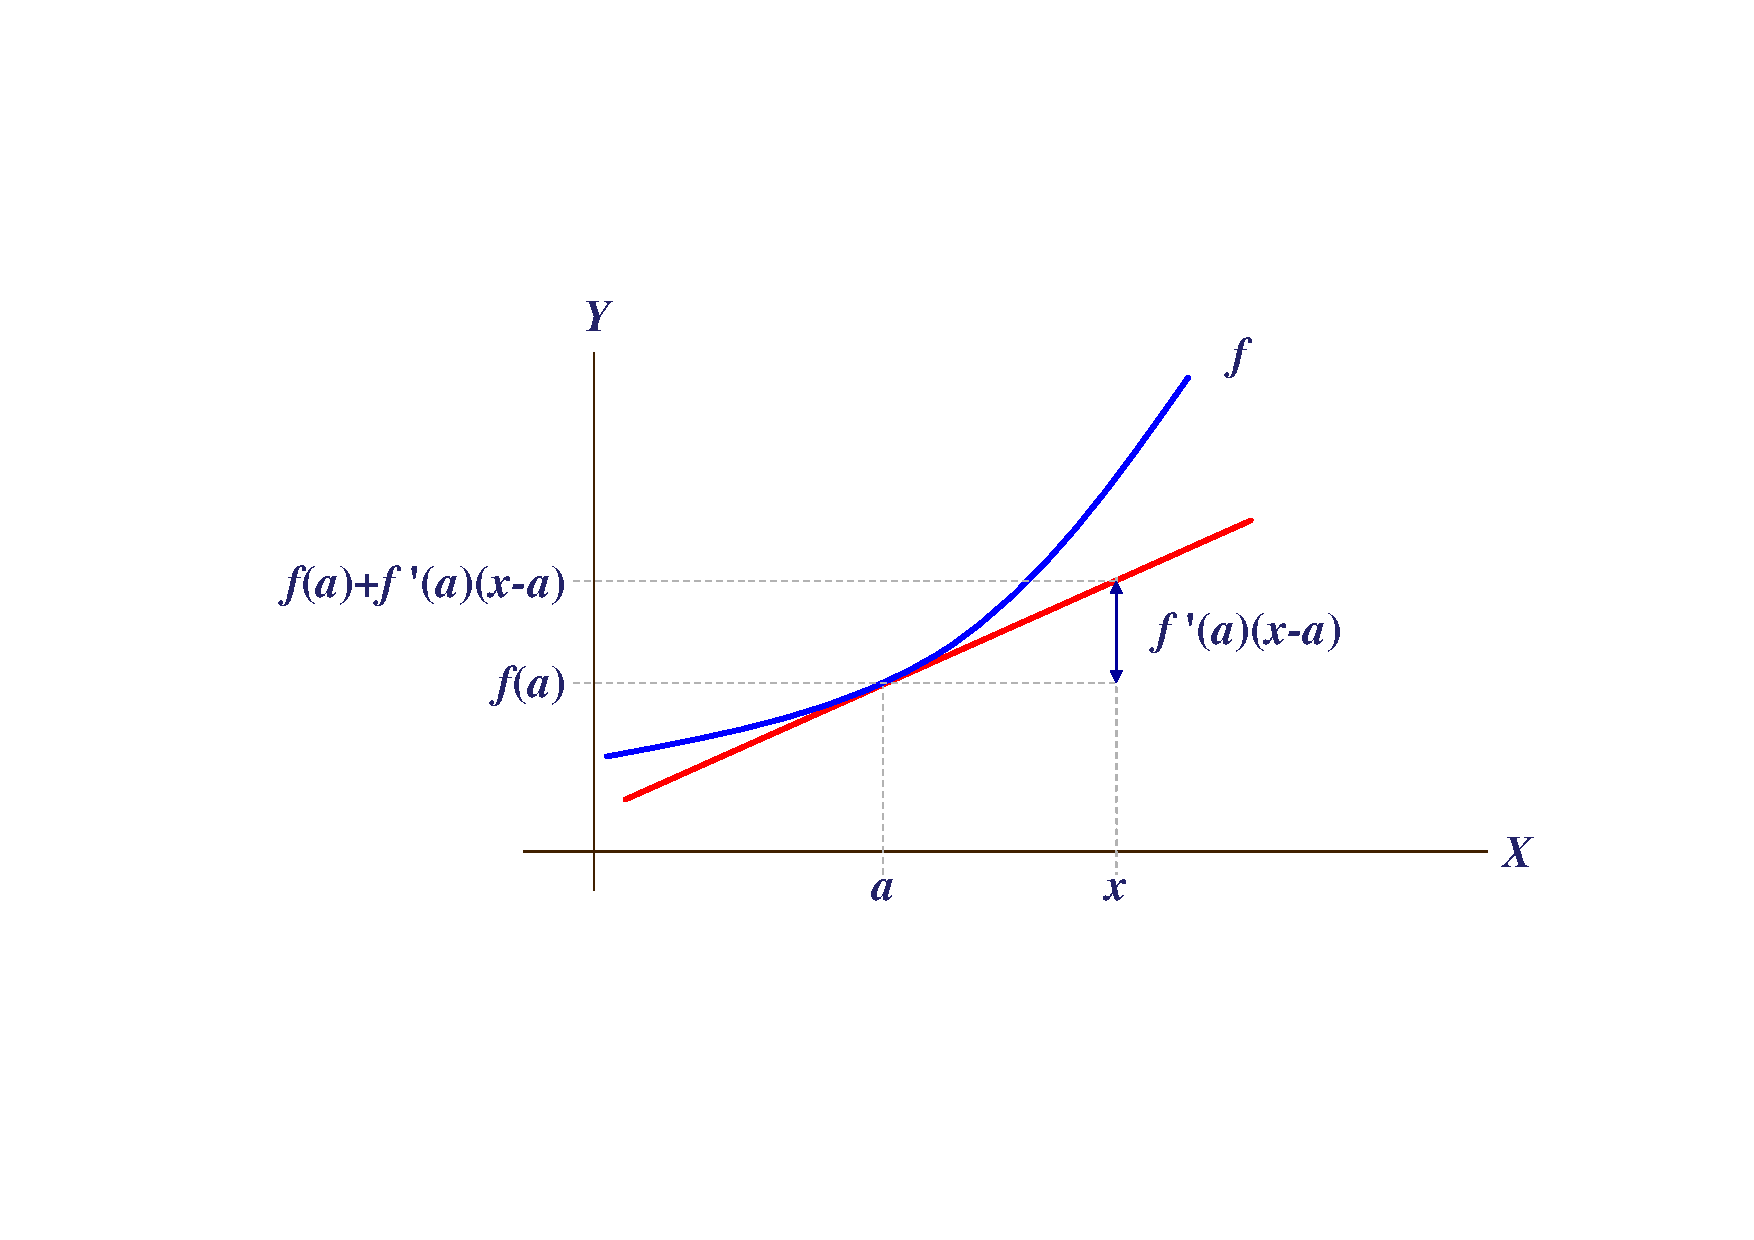
\includegraphics[scale=0.5]{tangente}
\caption{La derivada como la pendiente de la 
recta tangente a una función en un punto.}
\label{g:tangente}
\end{center}
\end{figure}


El límite anterior define una nueva función $f'$ cuyo dominio está formado por los
puntos en los que $f$ es diferenciable. La función $f'$ se llama \emph{primera
derivada} de $f$. Puesto que $f'$ es una función, puede derivarse a su vez, y a
la primera derivada de $f'$ se le conoce como segunda derivada de $f$, y se
nota $f''(x)$ o $\dfrac{d^2f}{dx^2}$. Análogamente, la \emph{$n$-ésima
derivada} de $f$, designada por $f^{(n}$ o $\dfrac{d^nf}{dx^n}$, es la primera
derivada de $f^{(n-1}$, para $n=2,3,\ldots$, es decir
\[
\frac{d^nf}{dx^n}=\frac{d}{dx}\left(\frac{d^{n-1}f}{dx^{n-1}}\right)\
n=2,3,\ldots
\]

\subsubsection*{Recta tangente y normal a una función en un punto}
Teniendo en cuenta lo anterior, la ecuación de la recta tangente a una función
$f(x)$ en el punto $(a,f(a))$ es
\[
y=f(a)+f'(a)(x-a).
\]
Del mismo modo, la ecuación de la recta normal a $f(x)$ en el punto $(a,f(a))$
es
\[
y=f(a)-\frac{1}{f'(a)}(x-a).
\]


\section*{Ejercicios Prácticos}
\begin{enumerate}[leftmargin=*]
\item Dada la función $f(x)=\dfrac{x^3+x^2-2x-2}{x+3}$, se pide:
\begin{enumerate}
\item Calcular la tasa de variación media de $f$ en los intervalos $[-1,3]$, $[-1,0]$ y $[-1,-0.5]$, y calcular las correspondientes rectas secantes. 
\item Calcular la tasa de variación instantánea de $f$ en el punto $-1$ haciendo uso de límites,y calcular la correspondiente recta tangente.
\end{enumerate}

\item Estudiar mediante la definición de derivada la derivabilidad de las funciones
siguientes (menú \texttt{Calculus->Limit} e introducir la expresión de la definición de derivada):


\[
f(x)=|x-1| \quad \textrm{en $x=1$,}
\]
\[
g(x)=\left\{%
\begin{array}{ll}
   x \sen\dfrac{1}{x}, & \hbox{si $x\neq 0$;} \\
   0, & \hbox{si $x=0$.} \\
\end{array}%
\right. \quad \textrm{en $x=0$.}
\]

\item  Calcular las derivadas de las siguientes funciones hasta el orden 4 (menú  \texttt{Calculus->} \texttt{Differentiate} y escribir el orden de la derivada en el cuadro \texttt{Order}):

\begin{enumerate}
\item  $a^x\log a$.

\item  $\dfrac{\sen x +\cos x}{2}$.

\item  $\dfrac{1}{\sqrt{1+x}}$.
\end{enumerate}

A la vista de los resultados, ¿cual sería la expresión de la
derivada $n$-ésima de cada una de estas funciones?

\end{enumerate}

\section*{Problemas}
\begin{enumerate}[leftmargin=*]

\item Una circunferencia metálica de radio 10 cm  se somete a un proceso de calentamiento en el que aumenta su radio 2 cm por segundo. ¿Cuál será la tasa de variación media del área del círculo a los 5 segundos? ¿Cuál será la tasa de variación instantánea del area del círculo en el instante inicial en que comienza a calentarse?

\item  Probar que no es derivable en $x=0$ la siguiente función:
\[ f(x)=\left\{
\begin{array}{ccl}
    e^x-1 &  & \mbox{si } x\geq 0,  \\
    x^3 &  & \mbox{si } x<0.
\end{array}\right.
\]

\item  Para cada una de las siguientes curvas, hallar las ecuaciones
de las rectas tangente y normal en el punto $x_{0}$ indicado.
\begin{enumerate}
    \item  $y=x^{\sen x},\quad x_{0}=\pi/2$.

    \item  $y=(3-x^2)^4\sqrt[3]{5x-4},\quad x_{0}=1$.

    \item  $y=\log \sqrt{\dfrac{1+x}{1-x}}+\arctg x, \quad x_{0}=0$.
\end{enumerate}

\end{enumerate}

\end{document}
